\section{Ikke elektroniske dele}
I dette afsnit gennemgås produktionen af de ikke-elektriske dele af produktet og mikrocontrollerprintet.

\subsection{Production af kanontårn}
Hele den fjernstyret kanon er holdt sammen af et kanontårn. Dette “skelet” er lavet af MDF (Medium Density Fiberboards) plader. Der er i alt fire forskellige plader. To af pladerne bruges som bunde, som skaber rotation om z-aksen. De sidste to plader fungerer som arme, som griber rundt om våbnet. Disse arme tillader rotation om x/y-aksen. \\

\begin{figure}[H]
\centering
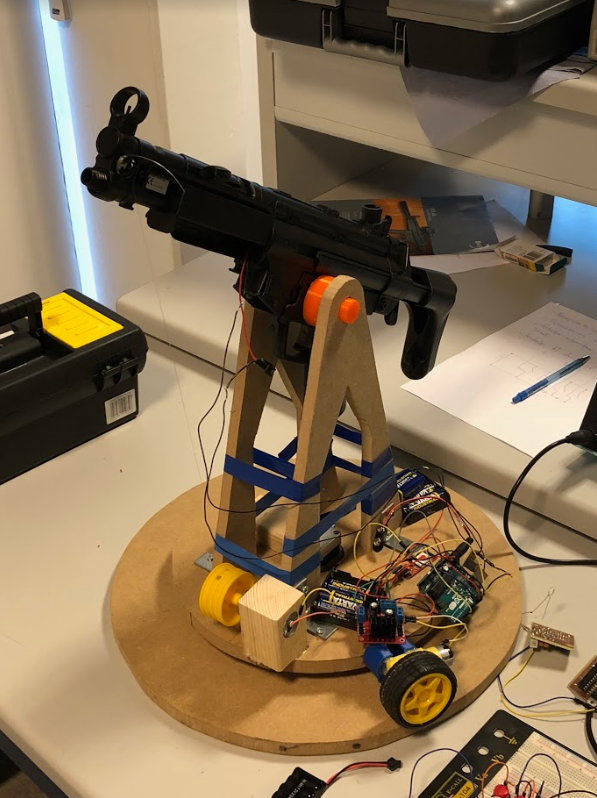
\includegraphics[scale=0.4]{Billeder/Kanontarn.PNG}
\caption{Det faerdiglavet produkt hvor skelettet kan ses.}
\label{fig:Kanontarn_faerdig}
\end{figure}

De fire plader er designet på sådanne måde, at de skal veje så lidt som muligt. De er blevet designet på sådanne måde, da motoren som sørger for rotation om z-aksen er mere effektiv, jo mindre vægt den skal flytte. Derudover er skelettet designet rundt om hardball-våbnet BT5\footnote{\url{https://www.legbilligt.dk/shop/14-el-gevaer---billige-softguns/238-bt---bt5-a5-kompletsaet/}} , som monterers på skelettet. 

\subsection{Production af 3D print}
Ud over de fire MDF plader er der også blevet produceret 3D-printet komponenter til kanontårnet. Alle de 3D-printede komponenter er lavet i Autodesk Fusion 360. \\

Alle de 3D-printede komponenter er designet til at hjælpe motoren med at roterer. \\

\begin{figure}[H]
\centering
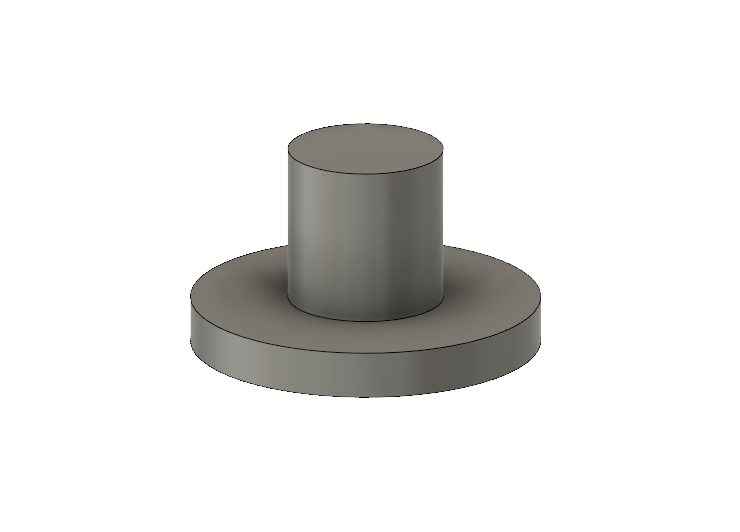
\includegraphics[scale=0.4]{Billeder/3D_print_1.PNG}
\caption{3D-print som hjaelper med x/y-rotation.}
\label{fig:3D_print_1}
\end{figure}

Dette komponent kan findes på begge sider af den monteret hardball pistol. Dette komponent hjælper med rotationen om x/y-aksen. \\

\begin{figure}[H]
\centering
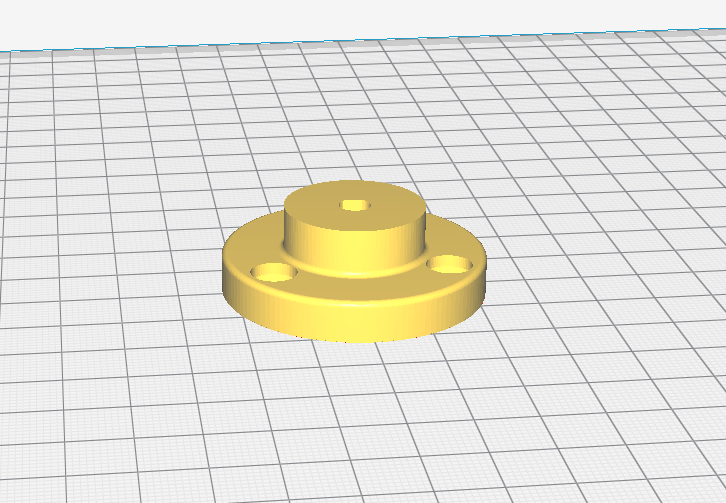
\includegraphics[scale=0.4]{Billeder/3D_print_2.PNG}
\caption{3D-print som hjaelper med z-rotation.}
\label{fig:3D_print_2}
\end{figure}

Dette komponent kan findes mellem de to MDF bundplader og hjælper med rotation om z-aksen.  \\

\subsection{Production af mikrocontrollerprint}

\begin{figure}[H]
\centering
\includegraphics[scale=0.4]{Billeder/Printpapir.jpg}
\caption{ Det gennemsigtige papir, som blev brugt til maalrettet belysning af kobberpladen.}
\label{fig:mikrocontrollerprint}
\end{figure}


Printet er anmærket ved at belyse en kobberplade dækket med lysfølsomt materiale gennem et gennemsigtigt papir, hvor kredsløbet er anmærket (se figur \ref{fig:mikrocontrollerprint}).\\


Printet er herefter blevet nedsænket i en svag natriumhydroxidopløsning, der kun fjerner den lysfølsomme belægning fra det belyste område. Dette gør, at når printet herefter nedsænkes i et syrebad, vil kun det kobber, hvorfra det ekstra lysfølsomme lag er opløst, blive ætset væk. Når dette er sket placeres printet i en stærkere natriumhydroxidopløsning, så resten af det lysfølsomme lag forsvinder. 






